% You must use only one of the following `\documentclass' commands
% For deliverables D2 and D3 you must use the following command:
%
\documentclass[runningheads,a4paper,oribibl]{llncs}
%
%For all other deliverables 
% you must use the command below (and put the one above in comments).
% 
%
%\documentclass[runningheads,a4paper]{llncs}

\usepackage[T1]{fontenc}  %% needed for special characters (umlaut)
\usepackage[latin1]{inputenc}
\usepackage{graphicx}     %% for graphical things such as including pictures
\usepackage{url}          %% for proper formatting of URLs
\usepackage{tikz}
\usepackage{float}
\usetikzlibrary{arrows, positioning}

\newcommand{\modelgit}{\texttt{github.com/}\allowbreak\texttt{serac01/}\allowbreak\texttt{hate-speech-detection-system}}
\newcommand{\modelone}{\texttt{cardiffnlp/}\allowbreak\texttt{twitter-}\allowbreak\texttt{roberta-}\allowbreak\texttt{base-}\allowbreak\texttt{hate}}
\newcommand{\modeltwo}{\texttt{unitary/}\allowbreak\texttt{unbiased-}\allowbreak\texttt{toxic-}\allowbreak\texttt{roberta}}

\begin{document}

\pagestyle{headings}

\mainmatter

\title{Dialectal Bias in Hate Speech Detection Systems}
\titlerunning{Dialectal Bias in Hate Speech Detection Systems}

\author{S\'{e}rgio Apolin\'{a}rio da Costa}

\institute{
    Department of Computing Science \\
    Ume\aa{} University, Sweden \\
    \email{mai25sca@cs.umu.se}
}

\maketitle

\begin{abstract}
This project audits two openly available classifiers, a hate speech detector and a toxicity detector, on
three Twitter corpora: Davidson et al., the Twitter part of HateXplain and the US random sample
of HateDay. Tweets are grouped by how closely their wording matches African-American English
(AAE) with the dialect model of Blodgett et al. On tweets that humans labelled 
\emph{neither hate nor offensive}, the AAE-aligned group is flagged more often by both classifiers
in all three corpora (false positive rate gaps from $+0.02$ to $+0.30$, all intervals above 
zero), and a random AAE-aligned tweet gets a higher score than a random mainstream one with
probability $0.62$ to $0.75$.
\end{abstract}

\section{Introduction}
Social media platforms rely on automatic classifiers to flag hateful content. This systems are
usually trained and tested on text close to mainstream written English. Friedman and Nissenbaum
call a system biased when it works well for the population it was built and tested on, but fails
for users who differ from it. African-American English (AAE) is a rule-governed variety of English
with its own grammar and vocabulary. Earlier work found that hate speech datasets, and the models
trained on them, treat tweets associated with AAE differently. This project audits two
openly available classifiers, on three different datasets.

\subsection{Research Questions}
This project will address the following research questions:
\begin{itemize}
  \item Do the classifiers flag AAE-aligned tweets that are \emph{not} hate more often than mainstream tweets?
  \item Does the gap appear for both classifiers, not only one?
  \item Does the gap appear in all three corpora?
  \item Does the gap stay when we use a different threshold?
  \item Does the gap stay when we define the groups in another way?
  \item Is the gap caused by the label mix of the two groups?
  \item Is the gap caused by profanity?
  \item Is the gap caused by tweet length?
  \item Do the words in the tweet explain the gap?
  \item Which words go with the false positives?
\end{itemize}
The hypothesis is that the classifiers flag more of the AAE-aligned tweets that are not hate
than of the mainstream ones.

\section{Literature Review}

\subsection{Automated Hate Speech Detection and the Problem of Offensive Language}
Davidson et al.~\cite{davidson2017} collected tweets that match a hate speech lexicon and had
crowd workers label them as \emph{hate speech}, \emph{offensive language} or \emph{neither}.
Their main point is that systems tend to confuse offensive language with hate speech. This
distinction is central here. A classifier may disagree with the labels because its definition
of hate differs, not because it is wrong. The main idea is that offensive language is not hate speech.

\subsection{Demographic Dialectal Variation in Social Media: A Case Study of AAE}
Blodgett et al.~\cite{blodgett2016} built a mixed-membership model from geolocated tweets and
Census demographics. For a tweet, it gives proportions over four demographically aligned language
groups, one of which is African-American-aligned. The output describes how much a text resembles
the usage of a group. It does not say who wrote it. In this project it is used as a measurement
instrument to split tweets into AAE-aligned and mainstream groups, and this limit is stated wherever it matters.

\subsection{The Risk of Racial Bias in Hate Speech Detection}
Sap et al.~\cite{sap2019} showed that AAE markers correlate with toxicity labels in hate speech
datasets, that classifiers trained on these data propagate the correlation, and that annotators
primed with dialect information label fewer tweets as offensive. Their results concern models
\emph{trained} on annotated corpora. In this project, it is used ready-made pretrained classifiers 
and it is evaluted on independent corpora. Following the usual reading of fairness as comparable
error rates across groups, it was used the false positive rate (FPR) as the main quantity.

\subsection{HateXplain: A Benchmark Dataset for Explainable Hate Speech Detection}
HateXplain~\cite{mathew2021} is a benchmark of about 20,000 posts from Twitter and Gab. It has
majority labels (hateful, offensive, normal), the targeted community and the words that justify
each label. This project uses its Twitter part as a second corpus, because the dialect model
was built on Twitter. It differs from Davidson in collection, annotation and text normalisation,
so a gap found in both is less likely to be a property of one dataset.

\subsection{HateDay: Insights from a Global Hate Speech Dataset Representative of a Day on Twitter}
HateDay~\cite{tonneau2024} is a random sample of all tweets posted on a single day (21 September
2022), annotated for hate speech. Unlike Davidson, which was selected with a lexicon, it reflects
what a platform actually sees. Most tweets are harmless and hate is rare. This project only uses
the US part as a third corpus to test whether the gap seen in lexicon-selected data also appears
in everyday tweets. The dataset is gated, so no tweet is printed, quoted or committed in this project.

\section{Materials and Methods}\label{sec:methods}

\subsection{Overview}
The pipeline, shown in Figure~\ref{fig:pipeline}, has four different stages.
Each stage is a group of scripts that writes files read by the next stage. The dialect model 
knows nothing about hate, the classifiers know nothing about dialect, and the human labels are
used only at evaluation. In this project it was not trained any model. The code is available on:
\modelgit\footnote{\url{https://github.com/serac01/hate-speech-detection-system}}.

\begin{figure}[htbp]
\centering
\resizebox{\textwidth}{!}{\hyphenpenalty=10000 \exhyphenpenalty=10000 %
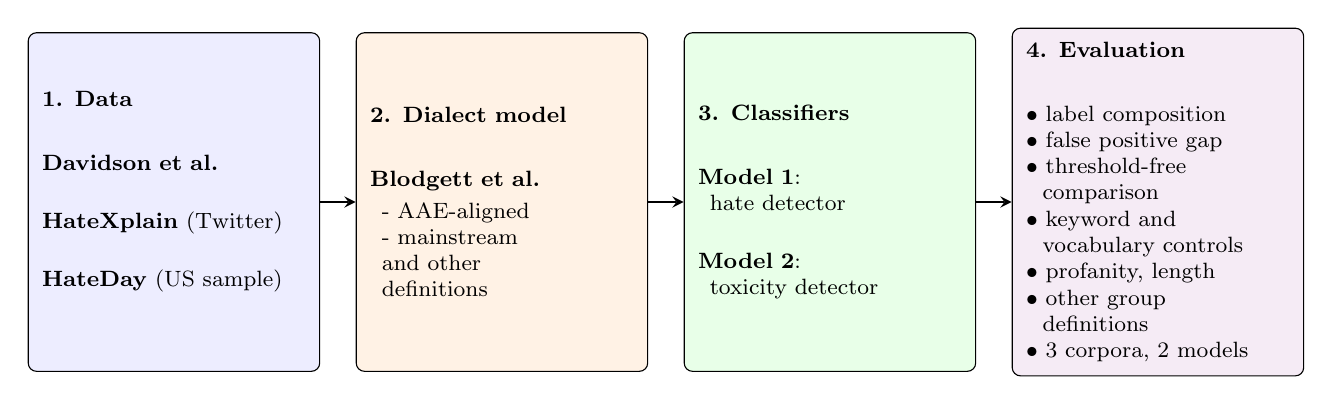
\begin{tikzpicture}[>=stealth, font=\footnotesize, node distance=0.45cm,
  stage/.style={draw, rounded corners=3pt, align=left, inner sep=5pt, text width=3.35cm, minimum height=4.3cm, anchor=north},
  arr/.style={->, thick}]

\node[stage, fill=blue!7] (s1) at (0,0) {{\bfseries 1. Data}\\ \hspace*{0.5em}\\[4pt]
  \textbf{Davidson et al.}\\ \hspace*{0.5em}\\[2pt]
  \textbf{HateXplain} (Twitter)\\ \hspace*{0.5em}\\[2pt]
  \textbf{HateDay} (US sample)\\ \hspace*{0.5em}\\[4pt]};

\node[stage, fill=orange!10, right=of s1] (s2) {{\bfseries 2. Dialect model}\\ \hspace*{0.5em}\\[4pt]
  \textbf{Blodgett et al.}\\[2pt]
  \hspace*{0.5em}- AAE-aligned\\
  \hspace*{0.5em}- mainstream\\
  \hspace*{0.5em}and other\\ \hspace*{0.5em}definitions};

\node[stage, fill=green!9, right=of s2] (s3) {{\bfseries 3. Classifiers}\\ \hspace*{0.5em}\\[4pt]
  \textbf{Model 1}:\\ \hspace*{0.5em}hate detector\\ \hspace*{0.5em}\\[2pt]
  \textbf{Model 2}:\\ \hspace*{0.5em}toxicity detector\\[4pt]};

\node[stage, fill=violet!8, right=of s3] (s4) {{\bfseries 4. Evaluation}\\ \hspace*{0.5em}\\[4pt]
  $\bullet$ label composition\\
  $\bullet$ false positive gap\\
  $\bullet$ threshold-free\\ \hspace*{0.7em}comparison\\
  $\bullet$ keyword and\\ \hspace*{0.7em}vocabulary controls\\
  $\bullet$ profanity, length\\
  $\bullet$ other group\\ \hspace*{0.7em}definitions\\
  $\bullet$ 3 corpora, 2 models};

\draw[arr] (s1.east) -- (s2.west);
\draw[arr] (s2.east) -- (s3.west);
\draw[arr] (s3.east) -- (s4.west);
\end{tikzpicture}}
\caption{Pipeline.\label{fig:pipeline}}
\end{figure}

\subsection{Data}
All the three datasets share the label coding: \emph{hate speech}, \emph{offensive language}, \emph{neither}.
The Davidson dataset has 24,783 tweets (1,430 hate, 19,190 offensive, 4,163 neither),
selected with a lexicon, so offensive vocabulary is over-represented.
The Twitter extracted section from the HateXplain dataset has 8,777 posts with a majority label
(normal = neither). Finnaly, the HateDay dataset with the US random sample has 26,970 tweets with
a single annotation each. This dataset is gated on Hugging Face, so no tweet is printed, quoted
or committed, and offensive words are masked in this report. The groups are estimated from the
text and the corpora have no author information.

\subsection{Dialect model}
The Blodgett et al.~\cite{blodgett2016} model was ported from Python 2 to 3 without changing inference.
The AAE score from the model is bag-of-words, so it is not the probability that an author is African
American. For this project it was setted a threshold for scoring, so a score $\geq0.6$ will be classified
as \emph{AAE-aligned} while a score  $\leq0.4$ will be classified as \emph{mainstream}. The rest
is excluded. As robustness it was used the argmax of the four-way posterior (AAE vs.\ White),
other thresholds, and a score computed after deleting profanity. This will be explored in more detail
in the next section.

\subsection{Classifiers}
Both classifiers run through Hugging Face with a threshold of 0.5 and 128 tokens.

The model 1, \modelone\footnote{\url{https://huggingface.co/cardiffnlp/twitter-roberta-base-hate}}, 
is a RoBERTa model pretrained on tweets and fine-tuned on the hate task of TweetEval, for example the
HatEval (SemEval 2019 Task 5: hate against immigrants and women, tweets collected in 2018). Its positive
class is \emph{hate}, so it is compared with \emph{hate speech}, the other two labels are negatives.

The model 2, \modeltwo\footnote{\url{https://huggingface.co/unitary/unbiased-toxic-roberta}}
is another RoBERTa model fine-tuned on the Jigsaw ``Unintended Bias in Toxicity Classification''
on comments (online news comments, not tweets). It detects \emph{toxicity}, not hate.
So, for this project the positive class was mapped to \emph{hate or offensive}. Its only real
negatives are the tweets labelled as \emph{neither}, and its flags on offensive tweets
are correct detections. This model was chosen after a first candidate (a Dynabench hate model)
was found to have been trained on data that includes Davidson's tweets, which would contaminate
the test, so it was replaced.

Both datasets are independence of the test data. The model 2 was trained on comments, so there
is no overlap with any tweet corpus by construction. The Model 1 was trained on 2018 HatEval
tweets. Davidson (collected 2017) and HateDay (2022) come from other collections. This is
independent by origin.

\subsection{Evaluation}\label{sec:evaluation}
The evaluation follows the steps of the notebook (Step~4). The two groups have very different label
mixes (Table~\ref{tab:mix}), so the first step is to show why overall error rates mislead, and
then compare the groups using the tweets labelled \emph{neither}, which are the true negatives
for both models.

\textbf{Main measures.} For each group it is computed the false positive rate (FPR) that is the
share of tweets that the model flags. The \emph{gap} is the FPR of the AAE-aligned group minus
the FPR of the mainstream group. A 95\% confidence interval for the gap comes from resampling
the tweets 2,000 times (bootstrap). Groups with fewer than 30 tweets are not evaluated.

\textbf{Steps.}
\begin{itemize}
  \item \emph{Step 4.1.1, baseline evaluation.} Precision, recall, F1 and FPR of each group,
    with the bootstrap gap.
  \item \emph{Step 4.1.2, flag rate within each label.} The share of tweets flagged inside each
    human label (neither, offensive, hate speech), and the gap after matching the label mix
    of the two groups.
  \item \emph{Step 4.1.3, comparison without the 0.5 threshold.} The $P(\mathrm{A}{>}\mathrm{M})$
    is the chance that a random AAE-aligned tweet gets a higher score than a random mainstream
    tweet (0.5 means no difference). It also give the FPR ratio, that measures how many times
    higher the AAE-aligned FPR is when the mainstream FPR is fixed at 10\%.
  \item \emph{Step 4.1.4, lexical controls.} A keyword control (women-directed profanity) and
    a vocabulary control (a bag-of-words model that predicts the flag from the words of the
    tweet).
  \item \emph{Step 4.1.5, other group definitions.} The same comparison with other ways of
    defining the groups.
  \item \emph{Steps 4.2 and 4.3, other corpora.} The same checks on HateXplain and HateDay.
    For HateDay it was added the controls for profanity and tweet length.
  \item \emph{Step 4.4, summary.} One table with the main result for the three corpora and
    the two models.
\end{itemize}

The confidence intervals only reflect sampling noise, not mistakes of the dialect model or of the human labels.

\section{Results}\label{sec:results}

\subsection{Baseline evaluation \emph{(Step 4.1.1)}}
Table~\ref{tab:mix} shows why a pooled comparison is misleading. 94.1\% of the AAE-aligned 
tweets are labelled offensive and only 2.0\% are labelled neither. In the mainstream group
the shares are 64.3\% and 28.2\%.
For model 1, F1 is the same in both groups (0.058 vs.\ 0.056, gap $+0.002$, CI $[-0.012,+0.015]$),
because the precision is about 0.03 in both. The FPR over all not-hate tweets is very different,
0.751 vs.\ 0.338 (gap $+0.412$, CI $[+0.397,+0.428]$). F1 hides the difference, which is why the
gap, and not the absolute error, is the finding.
For model 2, the positive class is hate or offensive, so its only false positives are the tweets
labelled neither. Its FPR is 0.253 vs.\ 0.161 (gap $+0.091$, CI $[+0.004,+0.180]$). Its F1 is
again equal in both groups (0.885 vs.\ 0.892, gap $-0.006$, CI $[-0.015,+0.002]$).

\begin{table}[H]
\centering\small\setlength{\tabcolsep}{3pt}
\resizebox{\textwidth}{!}{\begin{tabular}{|l|rr|rr|rr|}
\hline
 & \multicolumn{2}{c|}{\textbf{Label mix (\%)}} & \multicolumn{2}{c|}{\textbf{Model 1 flags (\%)}} & \multicolumn{2}{c|}{\textbf{Model 2 flags (\%)}} \\
Davidson label & AAE & Main. & AAE & Main. & AAE & Main. \\
\hline
Neither (FPR) & 2.0 & 28.2 & 9.5 & 1.6 & 25.3 & 16.1 \\
Offensive & 94.1 & 64.3 & 76.5 & 48.0 & 79.7 & 85.5 \\
Hate speech (recall) & 3.9 & 7.5 & 58.8 & 14.9 & 84.1 & 85.7 \\
\hline
\end{tabular}}
\caption{Davidson: label mix of the groups and share of tweets flagged by each model within each label.\label{tab:mix}}
\end{table}

\subsection{Flag rate within each label \emph{(Step 4.1.2)}}\label{sec:within}
Table~\ref{tab:mix} also gives the share of tweets flagged inside each human label. This removes
the effect of the different label mixes. These are descriptive rates, without confidence intervals.
The intervals come in Sect.~\ref{sec:groupdefs}.
Model 1 flags the AAE-aligned group more often in every label. 9.5\% vs.\ 1.6\% of the neither
tweets, 76.5\% vs.\ 48.0\% of the offensive tweets, and 58.8\% vs.\ 14.9\% of the hate speech
tweets. The gap is therefore not only a matter of label mix.
Model 2 is different. It flags the AAE-aligned group more often only for the neither tweets
(25.3\% vs.\ 16.1\%). For offensive tweets (79.7\% vs.\ 85.5\%) and hate tweets (84.1\% vs.\ 85.7\%),
which are correct detections for a toxicity model, it flags the AAE-aligned group slightly less
or equally often. The extra flags of model 2 are therefore on tweets that humans considered
harmless.

\subsection{Comparison without the threshold \emph{(Step 4.1.3)}}
Among the tweets that are not in the model's positive class (\emph{neither} and \emph{offensive}
for model 1, \emph{neither} for model 2), the $P(\mathrm{A}{>}\mathrm{M})$ is $0.761$
(CI $[0.753,0.768]$) for model 1 and $0.656$ ($[0.611,0.707]$) for model 2.
With the threshold set so that the mainstream group has an FPR of 10\%, the AAE-aligned group
has an FPR 3.0 (model 1) and 1.8 (model 2) times as high. The effect is therefore not a product
of the default threshold.

\subsection{Lexical controls \emph{(Step 4.1.4)}}\label{sec:words}
Model 1 was trained on a corpus that includes hate against women, so it may have learned to flag
women-directed profanity (b*tch, h*es), which is frequent in AAE-aligned tweets 
(91\% of the AAE-aligned offensive tweets contain one of 17 such terms vs.\ 77\%).

\textbf{Keyword control.} Among offensive tweets the gap of model 1 is $+0.225$ with a term and
$+0.054$ without (CIs $[+0.209,+0.241]$ and $[+0.023,+0.085]$). The terms matter a lot but do
not account for all of it. Among \emph{neither} tweets, adjusting for the share with a term
leaves the gap unchanged ($+0.078\to+0.076$), although almost none of those tweets contain a term. 

\textbf{Vocabulary control.} A cross-validated bag-of-words logistic regression predicts each
classifier's flag from the words of the tweet, on the tweets that are not labelled hate speech.
For model 1 it reproduces 89\% of the gap (residual $+0.046$, CI $[+0.035,+0.056]$; $+0.036$ to $+0.087$ across tokenizers and
regularisation). A ridge regression on the raw score leaves $+0.039$ (CI $[+0.032,+0.041]$).
For model 2 it reproduces 97\% (residual $+0.004$, CI $[-0.002,+0.011]$) because this subset
includes the offensive tweets, this is model 2's flag gap on non-hate tweets rather than its
false-positive gap. The words most often flagged are profanity, AAE markers (\emph{wit},
\emph{aint}, \emph{tryna}) and, for model 1, gendered words (\emph{she}, \emph{her}). One
spelling of the n-word is flagged in only 8.6\% of 116 tweets by model 1 while another is
flagged 77\% of the time (33.6\% vs.\ 97.7\% for model 2), so the models react to the form of
the word.  The groups are defined by words, so this control cannot tell dialect bias from
lexical bias.

\subsection{Gap within each label and other group definitions \emph{(Step 4.1.5)}}\label{sec:groupdefs}
The groups have a different label mix, so this project compares them inside each label. For the model 1,
the gap is $+0.285$ on offensive tweets (CI $[+0.269,+0.302]$) and $+0.078$ on \emph{neither}
tweets (CI $[+0.024,+0.141]$). When the mainstream group is given the same label mix, the gap
falls from $+0.412$ to $+0.281$ (CI $[+0.265,+0.296]$). So about two thirds of the gap is not
caused by the label mix.

Table~\ref{tab:groupdefs} uses other group definitions. With argmax and with profanity removed
before dialect scoring, the \emph{neither} gap stays above zero for both models. Stricter
thresholds leave too few \emph{neither} tweets, so it is used the re-weighted gap instead. For model 1
it grows to $+0.373$ ($0.7/0.3$) and $+0.501$ ($0.8/0.2$). Removing profanity lowers it to
$+0.166$, since many AAE-aligned tweets are in that group because of profanity. 

\begin{table}[H]
\centering\small\setlength{\tabcolsep}{3pt}
\resizebox{\textwidth}{!}{\begin{tabular}{|l|rrr|rr|}
\hline
 & \multicolumn{3}{c|}{\textbf{Model 1}} & \multicolumn{2}{c|}{\textbf{Model 2}} \\
Group definition (Davidson) & \emph{neither} gap & std.\ gap & $P(\mathrm{A}{>}\mathrm{M})$ & \emph{neither} gap & $P(\mathrm{A}{>}\mathrm{M})$ \\
\hline
Baseline 0.6 / 0.4 & $+.078$ [.024,.141] & $+.281$ & .674 & $+.091$ [.004,.180] & .656 \\
Argmax (AAE vs.\ White) & $+.031$ [.015,.049] & $+.310$ & .617 & $+.173$ [.135,.211] & .656 \\
Profanity removed before scoring & $+.084$ [.028,.142] & $+.166$ & .682 & $+.097$ [.005,.188] & .657 \\
Stricter 0.7 / 0.3 & -- & $+.373$ & -- & -- & -- \\
Stricter 0.8 / 0.2 & -- & $+.501$ & -- & -- & -- \\
\hline
\end{tabular}}
\caption{gap on \emph{neither} tweets (95\% CI), label-standardised gap on all not-hate
tweets, and $P(\mathrm{A}{>}\mathrm{M})$ on \emph{neither} tweets.\label{tab:groupdefs}}
\end{table}

\subsection{HateXplain and HateDay \emph{(Steps 4.2 to 4.4)}}\label{sec:three}
Table~\ref{tab:three} and Fig.~\ref{fig:pab} give the same quantities for the three corpora,
on the \emph{neither} tweets for both models. In all 12 rows the CI of the gap is above zero
and $P(\mathrm{A}{>}\mathrm{M})$ lies between 0.62 and 0.75. The absolute gaps differ by an
order of magnitude (HateDay $+0.01$ to $+0.07$, HateXplain $+0.17$ to $+0.31$) because the base
rate of flags differs between corpora. The $P(\mathrm{A}{>}\mathrm{M})$ and the FPR ratios 
(1.6 to 3.5 when the mainstream FPR is 10\%) are comparable across them.

\begin{table}[H]
\centering\footnotesize\setlength{\tabcolsep}{2.5pt}
\resizebox{\textwidth}{!}{\begin{tabular}{|l|c|r|c|c|c|r|}
\hline
Corpus, groups & Model & $n$ AAE / main. & FPR AAE / main. & Gap [95\% CI] & $P(\mathrm{A}{>}\mathrm{M})$ & flagged AAE \\
\hline
Davidson, baseline & 1 & 95 / 3,724 & 0.095 / 0.016 & $+0.078$ [0.025, 0.142] & 0.674 & 9 \\
 & 2 & 95 / 3,724 & 0.253 / 0.161 & $+0.091$ [0.002, 0.180] & 0.656 & 24 \\ \hline
Davidson, argmax & 1 & 626 / 2,688 & 0.046 / 0.015 & $+0.031$ [0.015, 0.049] & 0.617 & 29 \\
 & 2 & 626 / 2,688 & 0.331 / 0.158 & $+0.173$ [0.133, 0.210] & 0.656 & 207 \\ \hline
HateXplain, baseline & 1 & 263 / 4,950 & 0.369 / 0.121 & $+0.248$ [0.188, 0.308] & 0.749 & 97 \\
 & 2 & 263 / 4,950 & 0.764 / 0.460 & $+0.304$ [0.249, 0.357] & 0.700 & 201 \\ \hline
HateXplain, argmax & 1 & 1,047 / 3,744 & 0.288 / 0.114 & $+0.174$ [0.146, 0.202] & 0.657 & 302 \\
 & 2 & 1,047 / 3,744 & 0.712 / 0.405 & $+0.306$ [0.274, 0.337] & 0.705 & 745 \\ \hline
HateDay, baseline & 1 & 286 / 23,652 & 0.031 / 0.008 & $+0.024$ [0.006, 0.045] & 0.733 & 9 \\
 & 2 & 286 / 23,652 & 0.098 / 0.033 & $+0.065$ [0.031, 0.103] & 0.668 & 28 \\ \hline
HateDay, argmax & 1 & 2,436 / 16,075 & 0.020 / 0.008 & $+0.012$ [0.006, 0.017] & 0.667 & 48 \\
 & 2 & 2,436 / 16,075 & 0.061 / 0.037 & $+0.025$ [0.015, 0.035] & 0.641 & 149 \\ \hline
\end{tabular}}
\caption{Tweets labelled \emph{neither}: FPR in the AAE-aligned and mainstream groups, gap with bootstrap CI, $P(\mathrm{A}{>}\mathrm{M})$ and number of AAE tweets flagged.\label{tab:three}}
\end{table}

\begin{figure}[H]
\centering
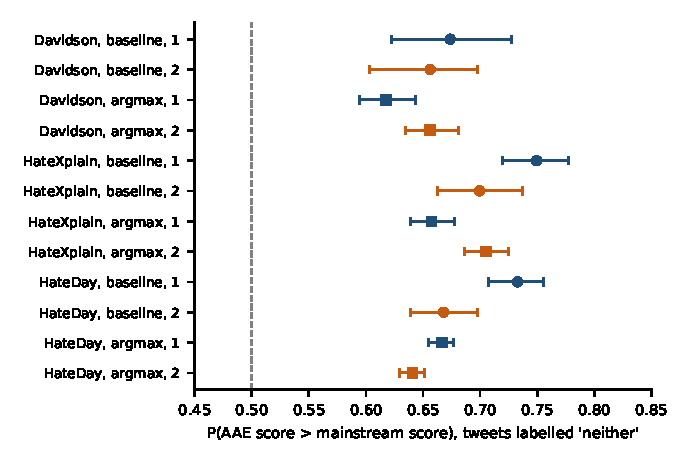
\includegraphics[width=0.78\textwidth]{fig_pab.pdf}
\caption{$P(\mathrm{A}{>}\mathrm{M})$ among \emph{neither} tweets with 95\% CI (circles: baseline groups; squares: argmax; blue: model 1; orange: model 2). All intervals lie above 0.5.\label{fig:pab}}
\end{figure}

\textbf{HateDay in detail.} HateDay is a random sample, and the results differ from Davidson.
The AAE-aligned group is small (397 tweets, 1.6\% of the sample) and has only 2 hate tweets,
so recall cannot be tested. Profanity is rare in both groups (4.9\% vs.\ 0.6\% of \emph{neither}
tweets), and AAE-aligned tweets are shorter (median 4 vs.\ 10 words). Even so, the gap remains
on tweets \emph{without} profanity ($+0.022$ [$+0.003,+0.043$] for model 1, $+0.033$
[$+0.006,+0.061$] for model 2) and after matching on length and profanity ($+0.023$ and $+0.040$).
It is smallest in very short tweets and grows with length. Unlike on Davidson, the vocabulary
explains only 12\% and 21\% of the flag gap (44\% and 37\% of the score gap). The words most tied
to the AAE-aligned group are harmless slang (\emph{fr, gm, nah, fam}) that is rarely flagged.
The model 1 gap rests on only 9 flagged AAE-aligned tweets, so $P(\mathrm{A}{>}\mathrm{M})$
is the more reliable number.

\section{Discussion}

\subsection{Answers to the research questions}

\begin{enumerate}
\item \textbf{Are AAE-aligned tweets that are not hate flagged more often?} Yes. On Davidson,
model 1 flags 9.5\% of the AAE-aligned \emph{neither} tweets and 1.6\% of the mainstream ones;
model 2 flags 25.3\% and 16.1\%. The AAE-aligned tweets also get higher scores. A random
AAE-aligned tweet scores higher than a random mainstream one with probability 0.62 to 0.75.
F1 and accuracy hide this, because F1 is the same in both groups.

\item \textbf{Does it happen for both classifiers?} Yes. The gap is positive, with a confidence
interval above zero, for model 1 (hate detector) and for model 2 (toxicity detector) in every
comparison. It is therefore not specific to one model or to one definition of harmful content.

\item \textbf{Does it happen in all three corpora?} Yes, in all 12 comparisons (3 corpora,
2 models, 2 group definitions). The size of the gap differs a lot: from $+0.01$ to $+0.07$ on
HateDay and from $+0.17$ to $+0.31$ on HateXplain. This is because the corpora have very
different shares of flagged tweets. $P(\mathrm{A}{>}\mathrm{M})$, which does not depend on
that share, is similar in all three (0.62 to 0.75).

\item \textbf{Does it stay with a different threshold?} Yes. $P(\mathrm{A}{>}\mathrm{M})$ uses
no threshold and is above 0.5 in all rows. When the threshold is set so that the mainstream
group has an FPR of 10\%, the AAE-aligned FPR is 1.6 to 3.5 times higher. The gap is not
caused by the default threshold of 0.5.

\item \textbf{Does it stay with other group definitions?} Yes. With argmax and with profanity
removed before dialect scoring, the gap on \emph{neither} tweets stays above zero for both
models. With stricter thresholds there are too few AAE-aligned \emph{neither} tweets, but the
re-weighted gap on all not-hate tweets grows (model 1: $+0.373$ and $+0.501$). The more clearly
a tweet matches AAE, the larger the gap.

\item \textbf{Is it caused by the label mix?} Only in part. On Davidson, 94\% of the AAE-aligned
tweets are offensive, against 64\% of the mainstream ones. When the mainstream group is given
the same label mix, the model 1 gap falls from $+0.412$ to $+0.281$. About a third of the gap
comes from the label mix, and two thirds remain. Inside each label the gap is still there
($+0.285$ on offensive tweets and $+0.078$ on \emph{neither} tweets).

\item \textbf{Is it caused by profanity?} In part on Davidson, not on HateDay. On Davidson,
profanity aimed at women matters a lot: among offensive tweets, the model 1 gap is $+0.225$
for tweets with such a word and $+0.054$ for tweets without. Removing profanity before dialect
scoring lowers the re-weighted gap to $+0.166$. On HateDay, profanity is rare, and the gap
remains on tweets without any profanity ($+0.022$ for model 1, $+0.033$ for model 2).

\item \textbf{Is it caused by tweet length?} No. This was tested on HateDay, where AAE-aligned
tweets are much shorter (median 4 vs.\ 10 words). After matching the groups on length and
profanity, the gap remains ($+0.023$ for model 1, $+0.040$ for model 2). The gap is smallest in
very short tweets and largest in long ones, so short length does not create the gap.

\item \textbf{Do the words explain the gap?} On Davidson, mostly yes: a bag-of-words model
reproduces 89\% (model 1) and 97\% (model 2) of the flag gap. On HateDay, mostly no: it
reproduces only 12\% and 21\% of the flag gap, and 44\% and 37\% of the score gap. However,
the groups are themselves defined by words, so this control cannot separate dialect bias from
word bias.

\item \textbf{Which words go with the false positives?} On Davidson: profanity, words aimed at
women, AAE words such as \emph{wit}, \emph{aint} and \emph{tryna}, and for model 1 also
\emph{she} and \emph{her}. The spelling matters: one spelling of the n-word is flagged by model
1 in 8.6\% of tweets, another in 77\%. On HateDay, the words most typical of the AAE-aligned
group are harmless slang (\emph{fr}, \emph{gm}, \emph{nah}, \emph{fam}), and they are rarely
flagged.

\end{enumerate}

\subsection{Further discussion}
The gap is robust, it appears for both models, in all corpora, at
any threshold and with any group definition. What causes it differs between corpora. On
Davidson, a lexicon-selected corpus, the flags mostly follow profanity and AAE words. On
HateDay, a random sample, words, profanity and length explain little of it. This suggests that
the models react to more than single words, but with only 9 flagged AAE-aligned tweets for
model 1 the evidence is thin.
Model 1 detects hate against immigrants and women,
model 2 detects toxicity, and Davidson separates hate from offensive language. These
differences can create a gap on their own. For example, model 1 probably learned to flag
profanity aimed at women, which is more common in AAE-aligned tweets. This is why the main
results use the \emph{neither} tweets, where no definition of hate applies. I read the gap as
a property of the systems as they are used, not as a finding about hate speech itself.

\textbf{Limitations.}
\begin{enumerate}
  \item The project only audits false positives. Recall cannot be tested on HateDay and is unreliable on the other corpora.
  \item The dialect score measures how similar the words are to AAE, not who wrote the
  tweet. Because the groups are defined by words, the word-based control cannot separate
  dialect bias from word bias. The baseline mainstream group also contains non-English tweets.
  \item The human labels are noisy. HateDay has one annotator per tweet, and the Davidson
  AAE-aligned \emph{neither} group is small (95 tweets).
  \item Toxicity is not hate, so the results for model 2 are about toxicity detection.
  \item Duplicates and retweets were not verified.
  \item The confidence intervals only cover sampling noise. They ignore errors of the dialect
  model and of the labels.
\end{enumerate}
A causal test would need the same content written in both AAE and mainstream English. No
such data exists for these corpora.

\section{The Final Report Compared with the Proposal}\label{sec:proposal}

\textbf{What was done.} The core of the proposal is done and extended. I compare AAE-aligned
and mainstream tweets with a pretrained classifier, labelled tweets and a dialect tool. I use
two classifiers instead of one, three corpora instead of one, bootstrap confidence intervals
and measures that do not depend on the threshold. The dialect tool of Blodgett et al.\ was
ported to Python 3 and, as planned, its score is treated as word similarity, not as the
identity of the author. The search for words tied to false positives is done.
Masking words and writing pairs of AAE and mainstream tweets were not done, because they need
new data. The expected outcome, that the classifier does worse on AAE tweets, is confirmed for
false positives. It is not visible in F1, and it cannot be tested for recall.

\textbf{What changed.} The proposal planned to use the Waseem and Hovy dataset. It is shared
only as tweet IDs, and downloading old tweets from the X API is no longer free (about \$95,
and many tweets are gone). Davidson includes the text, so it became the main corpus.
HateXplain and HateDay were added to test if the result holds on other data. HateDay is a
random sample, so it balances the lexicon-selected Davidson sample. The proposal also planned
to compare how well the model does on each group. Accuracy and F1 are not fair here, because
the classifiers definitions of hate differ from the labels (Table~\ref{tab:mix}). The FPR gap
became the main measure, as agreed with Rahil.

\textbf{What was not done.} Fine-tuning on a balanced sample was moved to future work, as
agreed with Rahil. Fine-tuning on Davidson would change the classifier's definition of
hate to Davidson's, so I couldn't tell a drop in bias from a change in what counts as hate.
This needs its own design. The time I had, on CPU only, went into the second classifier and
the random sample instead.

\textbf{Rahil feedback.}
\begin{itemize}
  \item \emph{Name the classifiers, their training data, and the label mapping.} Done in
  Sect.~\ref{sec:methods}. A first version of model 2 had been trained on Davidson's tweets,
  so it was replaced.
  \item \emph{Make sure the data is available.} Waseem and Hovy was replaced by Davidson.
  HateDay is gated, and none of its tweets is stored in the repository.
  \item \emph{Narrow the scope.} The work focuses on one question, the false positive gap,
  and on what explains it. Fine-tuning was dropped. I use one family of measures: the FPR
  gap and $P(\mathrm{A}{>}\mathrm{M})$.
  \item \emph{Use a second model.} Model 2 was added. The gap appears for both models
  (Sect.~\ref{sec:three}).
  \item \emph{State the definition mismatch (profanity aimed at women).} Discussed above and
  measured with the keyword control (Sect.~\ref{sec:words}).
  \item \emph{Compare the FPR within each label.} Done in Sect.~\ref{sec:within} and
  Sect.~\ref{sec:groupdefs}. The gap remains inside each label, and about a third of the
  overall gap comes from the label mix.
\end{itemize}

\textbf{Future work.}
\begin{itemize}
  \item Fine-tune on a sample balanced by dialect and class, and compare it with 
  changing the threshold per group, while keeping the definition of hate fixed.
  \item Mask the flagged words and run the classifiers again, and write pairs of the same
  tweet in AAE and mainstream English.
  \item Remove duplicates and retweets, check overlap with the training data at the text level,
  and read the flagged HateDay tweets by hand (without sharing them).
\end{itemize}

\section{Conclusion}
Two pretrained classifiers, one for hate and one for toxicity, flag AAE-aligned tweets that
humans labelled \emph{neither} more often than mainstream tweets. This happens in three corpora
and in all 12 comparisons. The label mix, the threshold and the way the groups are defined do
not remove the gap. On Davidson, the flags mostly follow the words in the tweet. On the random
sample, the gap is not explained by the words, but it rests on few flagged tweets. I cannot say
whether the classifiers react to the dialect itself, and I leave mitigation to future work.

\bibliographystyle{plain}
\bibliography{references}

\end{document}
